\documentclass{standalone}
\usepackage{tikz}
\usetikzlibrary{patterns, positioning}
\usepackage[sfdefault]{ClearSans} %% option 'sfdefault' activates Clear Sans as the default text font
\usepackage[T1]{fontenc}

\begin{document}
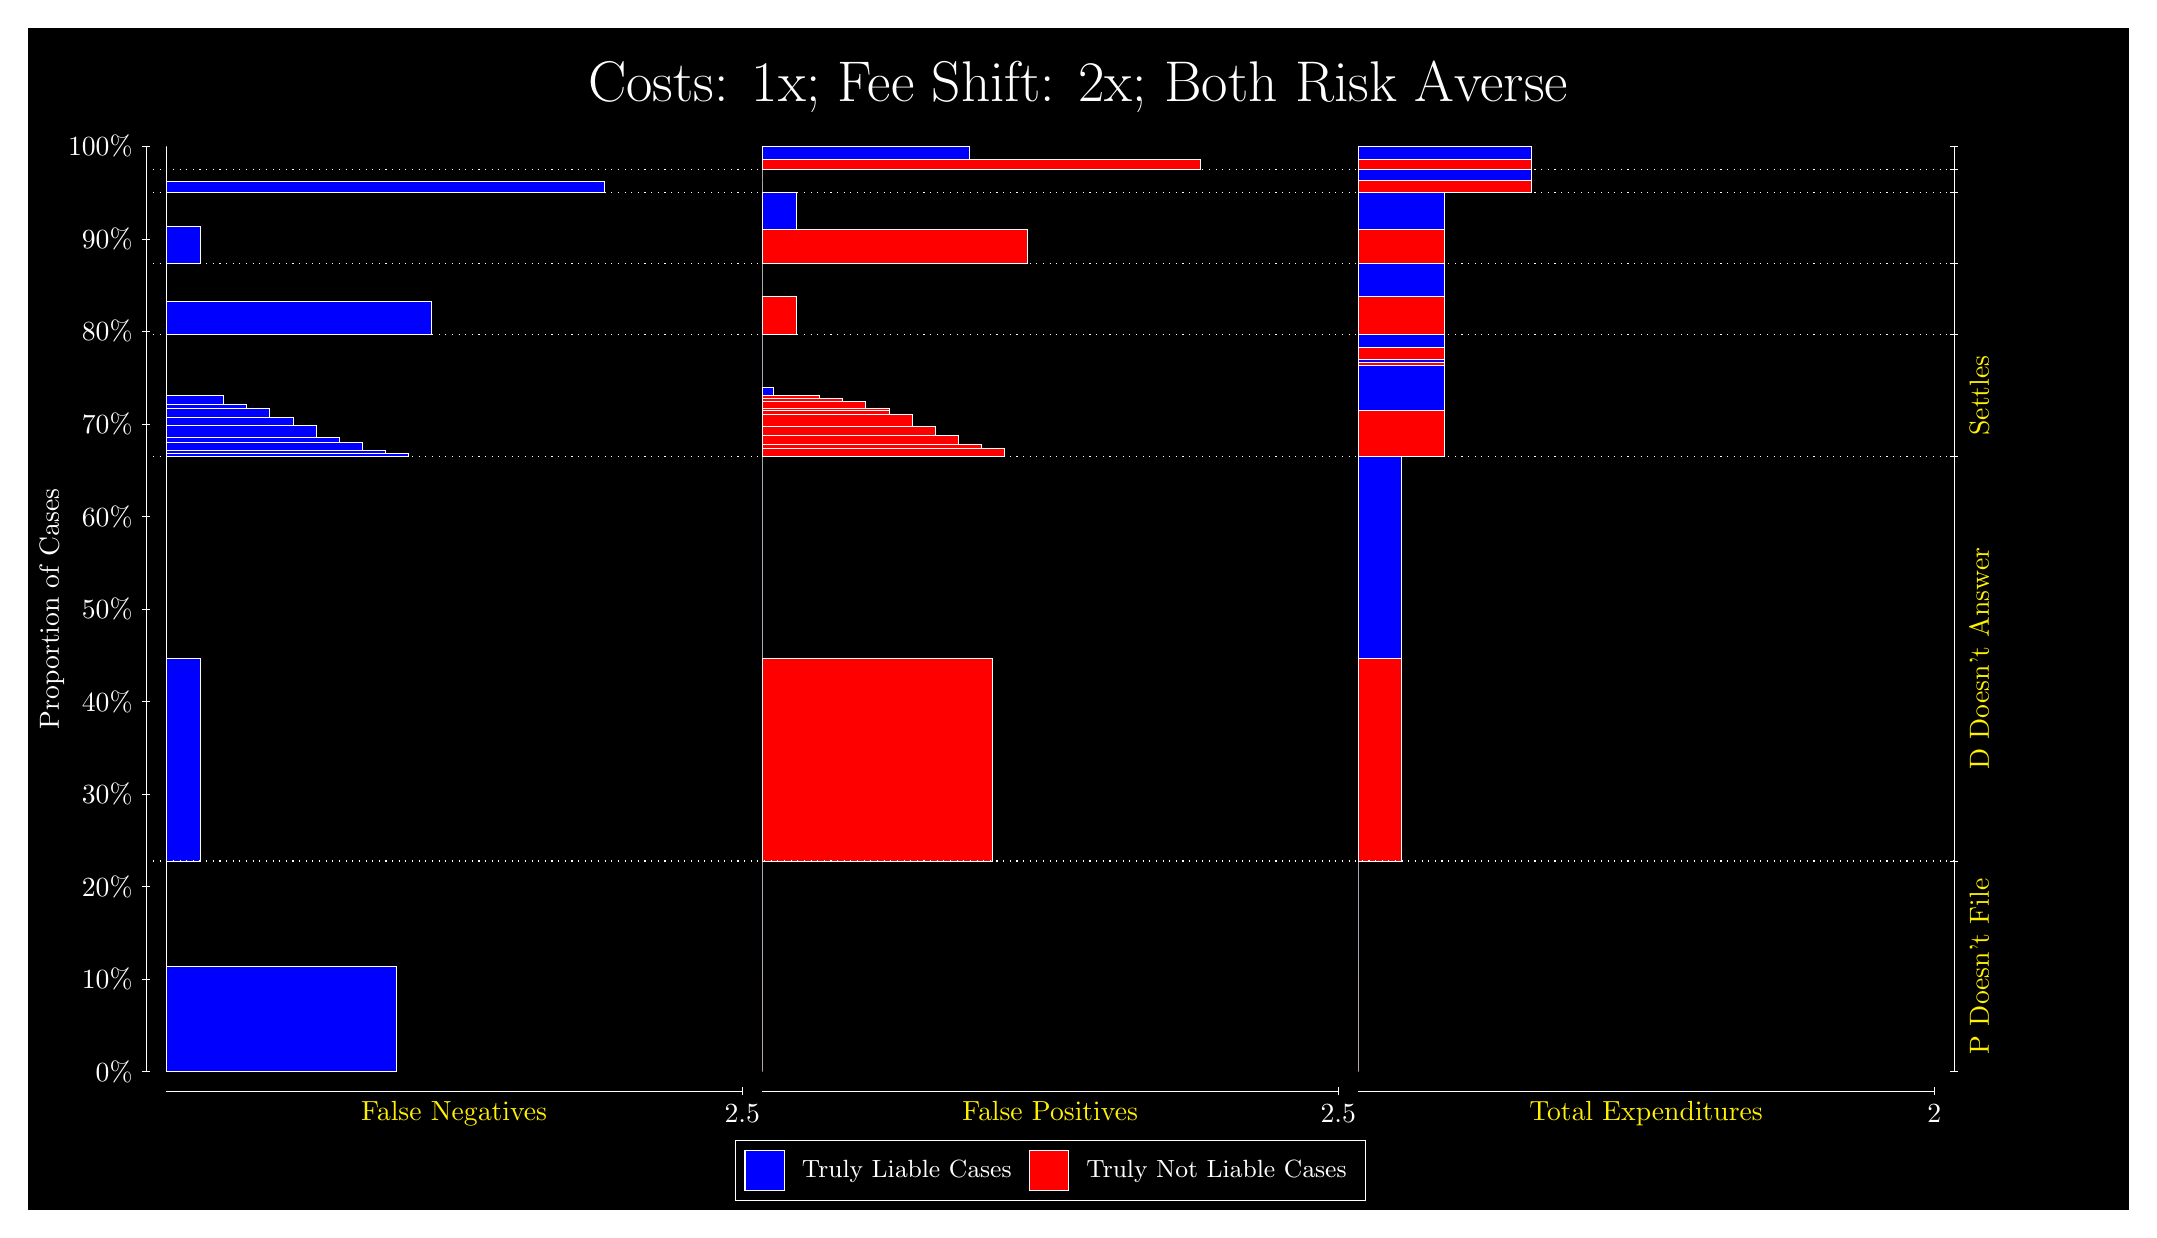
\begin{tikzpicture}
\draw[fill=black] (0,0) rectangle (26.667,15);
\draw[text=white] (0,13.5) rectangle (26.667,15) node[midway] {\huge Costs: 1x; Fee Shift: 2x; Both Risk Averse};
\draw[white, very thin] (1.5,1.75) -- (1.5,13.5);
\node[rotate=90, text=white, anchor=center] at (0.3, 7.625) {Proportion of Cases};
\draw[white, very thin] (1.45,1.75) -- (1.55,1.75);
\node[text=white, anchor=east] at (1.45, 1.75) {0\%};
\draw[white, very thin] (1.45,2.925) -- (1.55,2.925);
\node[text=white, anchor=east] at (1.45, 2.925) {10\%};
\draw[white, very thin] (1.45,4.1) -- (1.55,4.1);
\node[text=white, anchor=east] at (1.45, 4.1) {20\%};
\draw[white, very thin] (1.45,5.275) -- (1.55,5.275);
\node[text=white, anchor=east] at (1.45, 5.275) {30\%};
\draw[white, very thin] (1.45,6.45) -- (1.55,6.45);
\node[text=white, anchor=east] at (1.45, 6.45) {40\%};
\draw[white, very thin] (1.45,7.625) -- (1.55,7.625);
\node[text=white, anchor=east] at (1.45, 7.625) {50\%};
\draw[white, very thin] (1.45,8.8) -- (1.55,8.8);
\node[text=white, anchor=east] at (1.45, 8.8) {60\%};
\draw[white, very thin] (1.45,9.975) -- (1.55,9.975);
\node[text=white, anchor=east] at (1.45, 9.975) {70\%};
\draw[white, very thin] (1.45,11.15) -- (1.55,11.15);
\node[text=white, anchor=east] at (1.45, 11.15) {80\%};
\draw[white, very thin] (1.45,12.325) -- (1.55,12.325);
\node[text=white, anchor=east] at (1.45, 12.325) {90\%};
\draw[white, very thin] (1.45,13.5) -- (1.55,13.5);
\node[text=white, anchor=east] at (1.45, 13.5) {100\%};

\draw[white, very thin] (24.457,1.75) -- (24.457,13.5);
\draw[white, very thin] (24.407,1.75) -- (24.507,1.75);
\node[anchor=west] at (24.407, 1.75) {};
\draw[white, very thin] (24.407,4.4243) -- (24.507,4.4243);
\node[anchor=west] at (24.407, 4.4243) {};
\draw[white, very thin] (24.407,9.5636) -- (24.507,9.5636);
\node[anchor=west] at (24.407, 9.5636) {};
\draw[white, very thin] (24.407,11.108) -- (24.507,11.108);
\node[anchor=west] at (24.407, 11.108) {};
\draw[white, very thin] (24.407,12.017) -- (24.507,12.017);
\node[anchor=west] at (24.407, 12.017) {};
\draw[white, very thin] (24.407,12.913) -- (24.507,12.913);
\node[anchor=west] at (24.407, 12.913) {};
\draw[white, very thin] (24.407,13.205) -- (24.507,13.205);
\node[anchor=west] at (24.407, 13.205) {};
\draw[white, very thin] (24.407,13.5) -- (24.507,13.5);
\node[anchor=west] at (24.407, 13.5) {};

\draw[white, very thin, fill=blue] (1.75,1.75) rectangle (4.6775,3.0871);
\draw[white, very thin, fill=red] (1.75,3.0871) rectangle (1.75,4.4243);
\draw[white, very thin, fill=blue] (1.75,4.4243) rectangle (2.1891,6.994);
\draw[white, very thin, fill=red] (1.75,6.994) rectangle (1.75,9.5636);
\draw[white, very thin, fill=blue] (1.75,9.5636) rectangle (4.8239,9.6023);
\draw[white, very thin, fill=blue] (1.75,9.6023) rectangle (4.5312,9.6389);
\draw[white, very thin, fill=blue] (1.75,9.6389) rectangle (4.2384,9.7352);
\draw[white, very thin, fill=blue] (1.75,9.7352) rectangle (3.9457,9.8087);
\draw[white, very thin, fill=blue] (1.75,9.8087) rectangle (3.6529,9.9526);
\draw[white, very thin, fill=blue] (1.75,9.9526) rectangle (3.3602,10.063);
\draw[white, very thin, fill=blue] (1.75,10.063) rectangle (3.0674,10.179);
\draw[white, very thin, fill=blue] (1.75,10.179) rectangle (2.7746,10.227);
\draw[white, very thin, fill=blue] (1.75,10.227) rectangle (2.4819,10.334);
\draw[white, very thin, fill=red] (1.75,10.334) rectangle (1.75,11.108);
\draw[white, very thin, fill=blue] (1.75,11.108) rectangle (5.1167,11.532);
\draw[white, very thin, fill=red] (1.75,11.532) rectangle (1.75,12.017);
\draw[white, very thin, fill=blue] (1.75,12.017) rectangle (2.1891,12.488);
\draw[white, very thin, fill=red] (1.75,12.488) rectangle (1.75,12.913);
\draw[white, very thin, fill=blue] (1.75,12.913) rectangle (7.3123,13.052);
\draw[white, very thin, fill=red] (1.75,13.052) rectangle (1.75,13.205);
\draw[white, very thin, fill=red] (1.75,13.205) rectangle (1.75,13.336);
\draw[white, very thin, fill=blue] (1.75,13.336) rectangle (1.75,13.5);
\draw[white, very thin, fill=red] (9.3189,1.75) rectangle (9.3189,3.0871);
\draw[white, very thin, fill=blue] (9.3189,3.0871) rectangle (9.3189,4.4243);
\draw[white, very thin, fill=red] (9.3189,4.4243) rectangle (12.246,6.994);
\draw[white, very thin, fill=blue] (9.3189,6.994) rectangle (9.3189,9.5636);
\draw[white, very thin, fill=red] (9.3189,9.5636) rectangle (12.393,9.6676);
\draw[white, very thin, fill=red] (9.3189,9.6676) rectangle (12.1,9.7141);
\draw[white, very thin, fill=red] (9.3189,9.7141) rectangle (11.807,9.8318);
\draw[white, very thin, fill=red] (9.3189,9.8318) rectangle (11.515,9.9455);
\draw[white, very thin, fill=red] (9.3189,9.9455) rectangle (11.222,10.093);
\draw[white, very thin, fill=red] (9.3189,10.093) rectangle (10.929,10.144);
\draw[white, very thin, fill=red] (9.3189,10.144) rectangle (10.929,10.167);
\draw[white, very thin, fill=red] (9.3189,10.167) rectangle (10.636,10.263);
\draw[white, very thin, fill=red] (9.3189,10.263) rectangle (10.344,10.298);
\draw[white, very thin, fill=red] (9.3189,10.298) rectangle (10.051,10.337);
\draw[white, very thin, fill=blue] (9.3189,10.337) rectangle (9.4652,10.445);
\draw[white, very thin, fill=blue] (9.3189,10.445) rectangle (9.3189,11.108);
\draw[white, very thin, fill=red] (9.3189,11.108) rectangle (9.758,11.593);
\draw[white, very thin, fill=blue] (9.3189,11.593) rectangle (9.3189,12.017);
\draw[white, very thin, fill=red] (9.3189,12.017) rectangle (12.686,12.442);
\draw[white, very thin, fill=blue] (9.3189,12.442) rectangle (9.758,12.913);
\draw[white, very thin, fill=red] (9.3189,12.913) rectangle (9.3189,13.066);
\draw[white, very thin, fill=blue] (9.3189,13.066) rectangle (9.3189,13.205);
\draw[white, very thin, fill=red] (9.3189,13.205) rectangle (14.881,13.336);
\draw[white, very thin, fill=blue] (9.3189,13.336) rectangle (11.954,13.5);
\draw[white, very thin, fill=red] (16.888,1.75) rectangle (16.888,3.0871);
\draw[white, very thin, fill=blue] (16.888,3.0871) rectangle (16.888,4.4243);
\draw[white, very thin, fill=red] (16.888,4.4243) rectangle (17.437,6.994);
\draw[white, very thin, fill=blue] (16.888,6.994) rectangle (17.437,9.5636);
\draw[white, very thin, fill=red] (16.888,9.5636) rectangle (17.986,10.144);
\draw[white, very thin, fill=blue] (16.888,10.144) rectangle (17.986,10.719);
\draw[white, very thin, fill=red] (16.888,10.719) rectangle (17.986,10.759);
\draw[white, very thin, fill=blue] (16.888,10.759) rectangle (17.986,10.798);
\draw[white, very thin, fill=red] (16.888,10.798) rectangle (17.986,10.951);
\draw[white, very thin, fill=blue] (16.888,10.951) rectangle (17.986,11.108);
\draw[white, very thin, fill=red] (16.888,11.108) rectangle (17.986,11.593);
\draw[white, very thin, fill=blue] (16.888,11.593) rectangle (17.986,12.017);
\draw[white, very thin, fill=red] (16.888,12.017) rectangle (17.986,12.442);
\draw[white, very thin, fill=blue] (16.888,12.442) rectangle (17.986,12.913);
\draw[white, very thin, fill=red] (16.888,12.913) rectangle (19.083,13.066);
\draw[white, very thin, fill=blue] (16.888,13.066) rectangle (19.083,13.205);
\draw[white, very thin, fill=red] (16.888,13.205) rectangle (19.083,13.336);
\draw[white, very thin, fill=blue] (16.888,13.336) rectangle (19.083,13.5);
\draw[white, dotted] (1.5,4.4243) -- (24.457,4.4243);
\draw[white, dotted] (1.5,9.5636) -- (24.457,9.5636);
\draw[white, dotted] (1.5,11.108) -- (24.457,11.108);
\draw[white, dotted] (1.5,12.017) -- (24.457,12.017);
\draw[white, dotted] (1.5,12.913) -- (24.457,12.913);
\draw[white, dotted] (1.5,13.205) -- (24.457,13.205);
\draw[white, very thin] (1.75,1.5) -- (9.0689,1.5);
\node[text=yellow, anchor=north] at (5.4094, 1.5) {False Negatives};
\draw[white, very thin] (9.0689,1.45) -- (9.0689,1.55);
\node[text=white, anchor=north] at (9.0689, 1.45) {2.5};

\draw[white, very thin] (9.3189,1.5) -- (16.638,1.5);
\node[text=yellow, anchor=north] at (12.978, 1.5) {False Positives};
\draw[white, very thin] (16.638,1.45) -- (16.638,1.55);
\node[text=white, anchor=north] at (16.638, 1.45) {2.5};

\draw[white, very thin] (16.888,1.5) -- (24.207,1.5);
\node[text=yellow, anchor=north] at (20.547, 1.5) {Total Expenditures};
\draw[white, very thin] (24.207,1.45) -- (24.207,1.55);
\node[text=white, anchor=north] at (24.207, 1.45) {2};

\node[text=yellow, centered, rotate=90] at (24.777, 3.0871) {P Doesn't File};
\node[text=yellow, centered, rotate=90] at (24.777, 6.994) {D Doesn't Answer};
\node[text=yellow, centered, rotate=90] at (24.777, 10.336) {Settles};





\draw (12.978300999999998,1.5) node[draw=none] (baseCoordinate) {};
\begin{scope}[align=center]
        \matrix[scale=0.5, draw=white, below=0.5cm of baseCoordinate, nodes={draw}, column sep=0.1cm]{
            \node[rectangle, draw, minimum width=0.5cm, minimum height=0.5cm, fill=blue] {}; &
            \node[draw=none, font=\small, text=white] (B) {Truly Liable Cases}; &
            \node[rectangle, draw, minimum width=0.5cm, minimum height=0.5cm, fill=red] {}; &
            \node[draw=none, font=\small, text=white] (B) {Truly Not Liable Cases}; \\
            };
\end{scope}

\end{tikzpicture}
\end{document}